\documentclass[11pt,norsk]{article}
\usepackage[utf8]{inputenc}
\usepackage[T1]{fontenc}
\usepackage{babel}
\usepackage{amsmath}
\usepackage{amsfonts}
\usepackage{amsthm}
\usepackage[colorlinks]{hyperref}
\usepackage{listings}
\usepackage{color}
\usepackage{hyperref}
\usepackage{graphicx}
\usepackage{cite}

\definecolor{dkgreen}{rgb}{0,0.6,0}
\definecolor{gray}{rgb}{0.5,0.5,0.5}
\definecolor{daynineyellow}{rgb}{1.0,0.655,0.102}
\definecolor{url}{rgb}{0.1,0.1,0.4}

\lstset{frame=tb,
	language=Python,
	aboveskip=3mm,
	belowskip=3mm,
	showstringspaces=false,
	columns=flexible,
	basicstyle={\small\ttfamily},
	numbers=none,
	numberstyle=\tiny\color{gray},
	keywordstyle=\color{blue},
	commentstyle=\color{daynineyellow},
	stringstyle=\color{dkgreen},
	breaklines=true,
	breakatwhitespace=true,
	tabsize=3
}

\lstset{inputpath="C:/Users/Torstein/Documents/UiO/MatInf1100/Python programmer"}
\hypersetup{colorlinks, urlcolor=url}

\author{Torstein Solheim Ølberg}
\title{Svar på Oblig nr. 2 i MatInf1100}

\begin{document}
\maketitle
	\begin{center}
\Large \textbf{Oppgaver}
	\end{center}
		\paragraph{1.}
			\begin{flushleft}
Ved hjelp av en GPS har vi målt farten v til et objekt som beveger seg. Målingene er gjordt ved $N + 1$ tidspunkter $(t_i)_{i=0}^{N}$ slik at resultatet er en følge av tall-par $(t_i, v_i)_{i=0}^{N}$ der $v_i$ angir farten ved tidspunktet $t_i$.
			\end{flushleft}
			\subparagraph{a)}
				\begin{flushleft}
Gi en algoritme for å beregne en tilnærming til objektets aksellerasjon $a(t) = v'(t)$ ut fra de beregnede verdiene $(t_i, v_i)$ av farten.
				\end{flushleft}
				\begin{flushleft}
\textbf{Løsning:}
				\end{flushleft}
				\begin{flushleft}
					\begin{lstlisting}[frame=single]
for i = 0, 1, 2, ..., (lengden av v - 1):
	a[i] = (v[i+1] - v[i])/(t[i+1] - t[i])
					\end{lstlisting}
				\end{flushleft}
			\subparagraph{b)}
				\begin{flushleft}
Gi en algoritme for å beregne en tilnærming til objektets avstand $s(t)$ fra startpunktet ut fra de beregnede verdiene når $v(t) = s'(t)$ og $s(t_0) = 0$
				\end{flushleft}
				\begin{flushleft}
\textbf{Løsning:}
				\end{flushleft}
				\begin{flushleft}
					\begin{lstlisting}[frame=single]
for i = 0, 1, 2, ..., (lengden av v - 1):
	s[i+1] = s[i] + (v[i+1] + v[i])/2.*(t[i+1] - t[i])
					\end{lstlisting}
				\end{flushleft}
			\subparagraph{c)}
				\begin{flushleft}
Fila \\ \href{http://www.uio.no/studier/emner/matnat/math/MAT-INF1100/h16/obliger/running.txt}{http://www.uio.no/studier/emner/matnat/math/MAT-INF1100/h16/obliger/running.txt} er en logfil fra en løpetur, der vi på hver linje finner kommaseparerte tid/fart verdier. Du har lært at du kan lese inn verdiene fra denne fila inn i to vektorer $t$ og $v$ ved hjelp av følgende kode:
					\begin{lstlisting}[frame=single]
t = []
v = []
infile = open('running.txt','r')
for line in infile:
	tnext, vnext = line.strip().split(',')
	t.append(float(tnext))
	v.append(float(vnext))
infile.close()
					\end{lstlisting}
Last ned fila running.txt og kjør denne koden, og bruk algoritmen fra a) og b) til å lage to plott: Et der du plotter objektets aksellerasjon mot tid, og et der du plotter objektets avstand fra startpunktet mot tid.
				\end{flushleft}
				\begin{flushleft}
\textbf{Løsning:}
				\end{flushleft}
\lstinputlisting{oblig2_oppg1c.py}
\flushleft 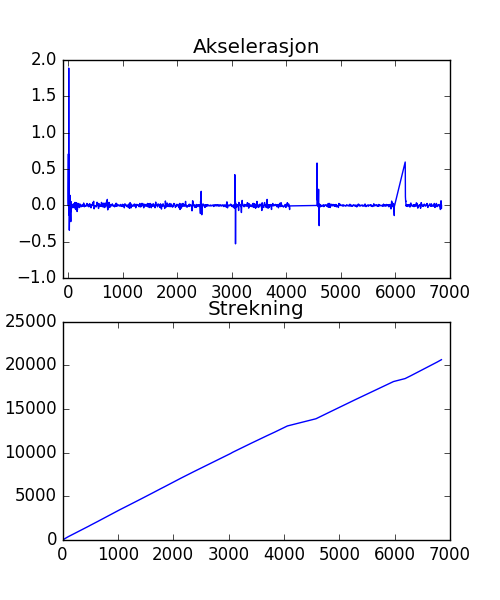
\includegraphics[width=13cm,height=11.9cm]{C:/Users/Torstein/Documents/UiO/MatInf1100/Python programmer/oblig2oppg1c.png}
		\paragraph{2.}
			\begin{flushleft}
Vi har differensialligningen
				\begin{align}\label{eq:difflig}
x' + x^2 = 1, \hspace{4mm} x(0) = 0.
				\end{align}
			\end{flushleft}
			\subparagraph{a)}
				\begin{flushleft}
Finn løsningen $x(t)$ av differensialligningen analystisk. (Hint: Ligningen er separabel.)
				\end{flushleft}
				\begin{flushleft}
\textbf{Løsning:}
				\end{flushleft}
				\begin{align}
x' + x^2 = 1 \\
x' = 1 - x^2 \\
\dfrac{x'}{1 - x^2} = 1 \\
\dfrac{\frac{dx}{dt}}{1 - x^2} = 1 \\
\int{\dfrac{dx}{1 - x^2}} = \int{1 dt} \\
\text{Integralet av $\frac{dx}{1 - x^2}$ er det samme som $arctanh(x)$ \hspace{0.01mm} (s.350 \cite{kalkulus})} \\
\text{som igjen er det samme som $\frac{1}{2}(ln(1 + x) - ln(1 - x))$} \nonumber \\
\dfrac{1}{2}(ln(1 + x) - ln(1 - x)) = t \\
\text{$ln(1 + x) - ln(1 - x)$ er det samme som $ln\Big{(}\frac{x + 1}{x - 1}\Big{)}$} \\
ln\Big{(}\frac{1 + x}{1 - x}\Big{)} = 2t \\
e^{ln(\frac{1 + x}{1 - x})} = e^{2t} \\
\dfrac{1 + x}{1 - x} = e^{2t} \\
x + 1 = - xe^{2t} + e{2t} \\
x + xe^{2t} = e^{2t} - 1 \\
\dfrac{x + e^{2t}}{1 + e^{2t}} = \dfrac{e^{2t} - 1}{e^{2t} + 1} \\
x = \dfrac{e^{2t} - 1}{1 + e^{2t}} 
				\end{align}
			\subparagraph{b)}
				\begin{flushleft}
Løs ligningen numerisk på intervallen $[0,2]$ ved å ta $5$ steg med Eulers metode (med kalkulator eller datamaskin). Plott den numeriske løsningen sammen med den eksakte løsningen (for hånd eller ved hjelp av datamaskin). 
				\end{flushleft}
				\begin{flushleft}
\textbf{Løsning:}
				\end{flushleft}
\lstinputlisting{oblig2_oppg2b.py}
\flushleft
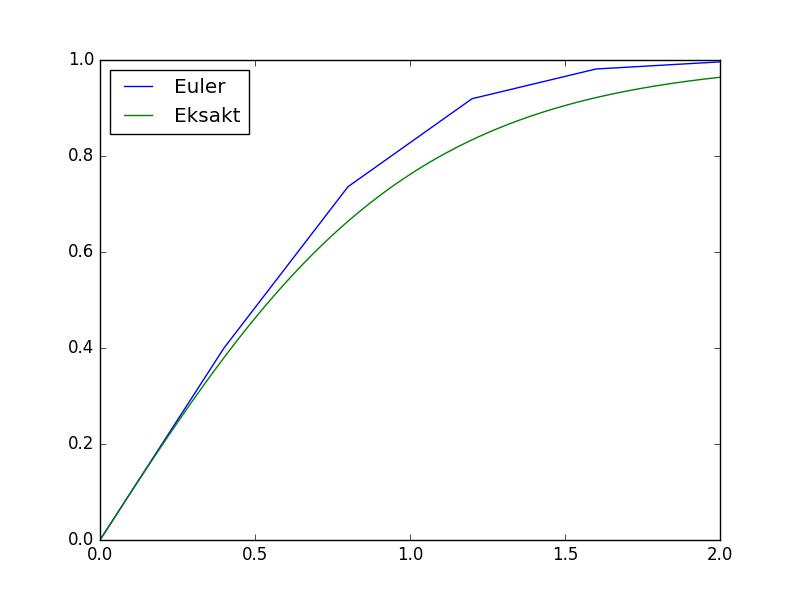
\includegraphics[width=8cm,height=8cm]{C:/Users/Torstein/Documents/UiO/MatInf1100/Python programmer/oblig2oppg2b.png}
			\subparagraph{c)}
				\begin{flushleft}
Gjenta (b), men bruk Eulers midpunktmetode i steden for Euler's metode. Plott den numeriske løsningen du nå får sammen med løsningene du plottet i (b).
				\end{flushleft}
				\begin{flushleft}
\textbf{Løsning:}
				\end{flushleft}
\lstinputlisting{oblig2_oppg2c.py}
\flushleft
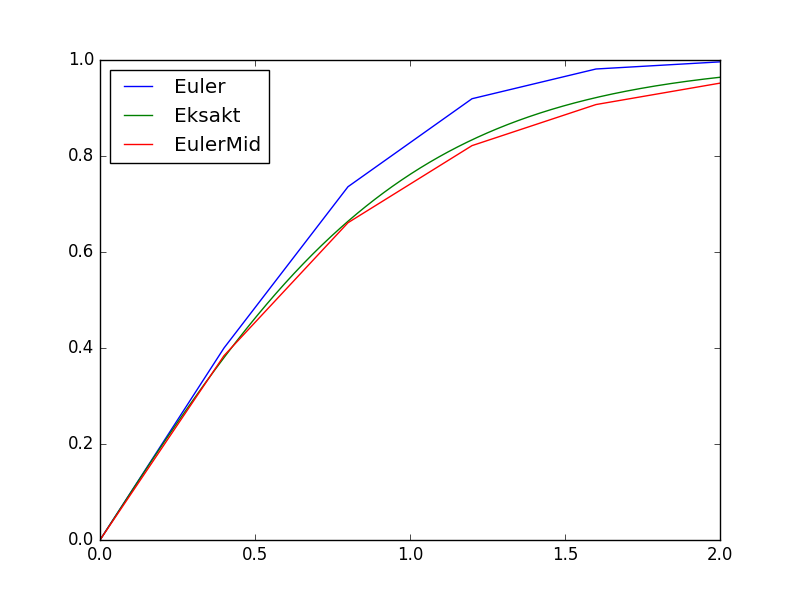
\includegraphics[width=8cm,height=9cm]{C:/Users/Torstein/Documents/UiO/MatInf1100/Python programmer/oblig2oppg2c.png}
			\subparagraph{d)}
				\begin{flushleft}
Anta at du vet at $0 \le x(t^{*}) \le 1$ for en verdi $t^{*}$. Bruk differensialligningen \eqref{eq:difflig} til å forklare at da vil $x(t)$ være voksende i $t = t^{*}$. Forsøk å utvide dette til å si noe om hvordan $x(t)$ oppfører seg om $x(t^{*}) > 1$ eller $x(t^{*}) = 1$. 
				\end{flushleft}
				\begin{flushleft}
\textbf{Løsning:}
				\end{flushleft}
				\begin{align}
0 \le x(t^{*}) < 1 \\
x' = 1 - x^2 \\
x'(t^{*}) = 1 - x(t^{*})^2 \Rightarrow 0 < x'(t^{*}) \le 1 \\
\text{Hvis $x(t^{*}) > 1$, så er:} \\
x'(t^{*}) = 1 - x(t^{*})^2 \Rightarrow x'(t^{*}) < 0 \hspace{2mm} \text{altså er avtakende.} \nonumber \\
\text{Hvis $x(t^{*}) = 1$ så er:} \\
x'(t^{*}) = 1 - x(t^{*})^2 \Rightarrow x'(t^{*}) = 0 \hspace{2mm} \text{altså $x(t)$ er konstant.} \nonumber
				\end{align}
			\subparagraph{e)}
				\begin{flushleft}
(Frivillig). Bruk differensialligningen \eqref{eq:difflig} til å vise at $x(t)$ er voksende for alle $t \ge 0$.
				\end{flushleft}
				\begin{flushleft}
\textbf{Løsning:}
				\end{flushleft}
				\begin{flushleft}
					\begin{align}
x' = 1 - x^2 \Rightarrow x'(t) = 1 - x(t)^2, t \ge 0 \nonumber
					\end{align}
Siden $x(t)$ er deriverbar for alle $t \ge 0$ er den kontinuerlig på intervallet $[0, \rightarrow)$ (Setning 6.1.9, s.259 \cite{kalkulus}). Da vet vi at siden likningen \eqref{eq:difflig} kan skrives på formen $\frac{x'(t)}{1 - x(t)^2} = 1$ så kan ikke $x(t)$ bli $1$ for noen $t$ fordi dette ville gitt divisjon med $0$. Noe som igjen betyr at $x'(t)$ ikke kan bli $0$ for noen $t$.
				\begin{align}
x'(t) = 1 - x(t)^2 \label{eq:deriv}\\
x''(t) = -2x(t)\cdot x'(t) \nonumber
				\end{align}
Av derivasjonen \eqref{eq:deriv} ser vi at den dobbeltderiverte til $x(t)$ bare avhenger av $x(t)$ og $x'(t)$, som begge eksisterer for alle $t$. På grunn av dette må $x''(t)$ også eksistere for alle $t$. Da kan vi konkludere med at også $x'(t)$ er kontinuerlig og siden $x'(t)$ ikke kan bli $0$, da dette vil bety at $x(t)$ må være $1$, så kan heller ikke $x'(t)$ bli negativ (Sjæringssetningen 5.2.1 s.221 \cite{kalkulus}) Siden $x'(t)$ ikke kan bli hverken $0$ eller negativ må den være positiv for alle $t \ge 0$ og da må $x(t)$ være voksende for alle $t \ge 0$.
				\end{flushleft}
	\begin{thebibliography}{9}
\bibitem{kalkulus}
Tom Lindstrøm.
\textit{Kalkulus 3.Utgave}.
Universitetsforlaget AS, Oslo, 2006
	\end{thebibliography}
\end{document}